\documentclass[conference,onecolumn]{IEEEtran}
\IEEEoverridecommandlockouts

% Essential Packages
\usepackage{cite}
\usepackage{amsmath,amssymb,amsfonts}
\usepackage{algorithmic}
\usepackage{graphicx}
\usepackage{textcomp}
\usepackage{xcolor}
\usepackage{booktabs}
\usepackage{listings}
\usepackage{tikz}
\usetikzlibrary{shapes.geometric, arrows.meta, positioning, shadows}
\usepackage{hyperref}
\usepackage{geometry}
\geometry{letterpaper, margin=1in}

% Code Listing Settings
\lstset{
    basicstyle=\ttfamily\footnotesize,
    breaklines=true,
    frame=single,
    backgroundcolor=\color{gray!8},
    keywordstyle=\color{blue}\bfseries,
    commentstyle=\color{green!50!black}\itshape,
    stringstyle=\color{purple},
    numbers=left,
    numberstyle=\tiny\color{gray},
    numbersep=5pt,
    tabsize=2,
    showstringspaces=false
}

\begin{document}

\title{Mitigating Algorithmic Sycophancy and Premature Consensus in Multi-Agent Scientific Hypothesis Generation via Persona Heterogeneity}

\author{\IEEEauthorblockN{Sarvagna Khatri - MSE2026005}

}

\maketitle

\begin{abstract}
Large language models (LLMs) are rapidly transforming scientific discovery by accelerating hypothesis generation—the formulation of novel, testable explanatory mechanisms from existing literature. While single-LLM pipelines leveraging chain-of-thought (CoT) and self-consistency provide strong, cost-effective baselines, multi-agent debate (MAD) frameworks have emerged to emulate collaborative scientific peer review. However, homogeneous multi-agent debate systems exhibit pathological failure modes: algorithmic sycophancy, the tyranny of the majority, and a insidious ``consistency illusion'' wherein agents converge toward superficial lexical consensus while degrading underlying reasoning alignment. In this study, we present a controlled, reproducible comparative evaluation measuring the impact of structural persona heterogeneity against a standard homogeneous multi-agent baseline on advanced biomedical and physical science topics (including ambient superconductivity and broad-spectrum antiviral targets). Using Gemini 1.5 Pro instances coordinated via round-robin debate and evaluated across Sentence-BERT semantic similarity spaces, we demonstrate that homogeneous agents degenerate into consensus within 1.35 rounds, exhibiting a high semantic overlap ($\sim 0.85$). In contrast, assigning deliberately polarized adversarial personas (The Domain Expert, The Speculative Theorist, and The Skeptical Reviewer) sustains productive debate across all scheduled rounds, decreases semantic overlap to $0.48$, and actively exposes methodological flaws. We release our experimental logs, evaluation suite, and audit records to establish reproducible benchmarks for agentic scientific exploration.
\end{abstract}

\begin{IEEEkeywords}
Multi-Agent Debate, Scientific Hypothesis Generation, Algorithmic Sycophancy, Consistency Illusion, Large Language Models, Persona Diversity, Sentence Transformers.
\end{IEEEkeywords}

\section{Introduction}
Scientific hypothesis generation has long been regarded as one of the least formalizable and most creative stages of the scientific method, heavily dependent on tacit domain expertise, interdisciplinary intuition, and iterative conjecture \cite{boiko2023autonomous}. Historically dominated by rule-based literature-based discovery, the recent deployment of frontier Large Language Models (LLMs) trained on broad scientific corpora has unlocked automated scientific ideation across chemistry, biology, and materials science \cite{boiko2023autonomous, swanson2025virtual}.

As LLM-driven research tools mature, two architectural paradigms have solidified:
\begin{enumerate}
    \item \textbf{Single-Agent Systems}: A single centralized foundation model orchestrates generation, augmented with retrieval-augmented generation (RAG), external API tool calling, or decoding-time sampling strategies such as self-consistency \cite{boiko2023autonomous}. Systems such as \textit{Coscientist} \cite{boiko2023autonomous} and early-stage idea benchmarks demonstrate that single models produce highly novel scientific concepts at modest computational expense.
    \item \textbf{Multi-Agent Deliberation and Debate (MAD)}: Multiple LLM instances, either homogeneous or role-differentiated, exchange natural language critiques over successive rounds to refine candidate hypotheses before rendering a final determination \cite{du2023improving, liang2024encouraging}. Notable systems such as \textit{SciAgents} \cite{ghafarollahi2025sciagents}, \textit{The Virtual Lab} \cite{swanson2025virtual}, and the \textit{AI Co-Scientist} \cite{gottweis2025towards} utilize specialized agent societies to explore combinatorial hypotheses across interdisciplinary domains.
\end{enumerate}

Despite the theoretical promise of multi-agent deliberation—originally grounded in AI safety via debate \cite{irving2018ai}—recent critical investigations reveal that multi-agent systems frequently suffer from systemic behavioral pathologies. Specifically, homogeneous multi-agent debate is prone to \textit{algorithmic sycophancy} and the \textit{tyranny of the majority}, where agents conform to peer assertions regardless of factual validity, collapsing into conversational echo chambers \cite{wynn2025talk}. In scientific discovery, this culminates in the ``consistency illusion'': agents appear to reach agreement on an empirical proposition, but the actual depth, diversity, and rigor of their collective reasoning degrade \cite{wynn2025talk}.

% ==========================================
% FIXED FIGURE 1 (Resized to fit text width)
% ==========================================
\begin{figure}[htbp]
\centering
\resizebox{\textwidth}{!}{%
\begin{tikzpicture}[
    node distance=1.5cm and 1.5cm,
    auto,
    block/.style={rectangle, draw=blue!70, fill=blue!10, rounded corners, text width=3.8cm, text centered, minimum height=1.3cm, drop shadow},
    roundblock/.style={ellipse, draw=red!70, fill=red!10, text width=3.0cm, text centered, minimum height=1.0cm, drop shadow},
    evalblock/.style={rectangle, draw=green!70, fill=green!10, text width=3.5cm, text centered, minimum height=1.2cm, drop shadow},
    arrow/.style={-Latex[length=3mm, width=2mm], thick, gray!80!black}
]

% Nodes
\node (prompt) [block] {\textbf{Research Input}\\ Domain Scientific Topic / Verification Challenge};
\node (homo) [roundblock, above right=0.8cm and 1.5cm of prompt] {\textbf{Homogeneous MAD}\\ $3\times$ Helpful AI Scientists};
\node (hetero) [roundblock, below right=0.8cm and 1.5cm of prompt] {\textbf{Heterogeneous MAD}\\ Expert, Optimist, Skeptic};
\node (homo_res) [block, right=1.5cm of homo] {\textbf{Baseline Trajectory}\\ Sycophantic Drift, Early Consensus ($R < 2$)};
\node (hetero_res) [block, right=1.5cm of hetero] {\textbf{Adversarial Trajectory}\\ Sustained Debate, High Divergence ($R = 3$)};

% Position eval directly between the two result blocks, shifted right
\path (homo_res) -- (hetero_res) coordinate[midway] (mid_res);
\node (eval) [evalblock, right=1.5cm of mid_res] {\textbf{Evaluation Engine}\\ S-BERT Divergence, Rounds, Failure Mode Tracking};

% Connections
\draw [arrow] (prompt) |- (homo);
\draw [arrow] (prompt) |- (hetero);
\draw [arrow] (homo) -- (homo_res);
\draw [arrow] (hetero) -- (hetero_res);
\draw [arrow] (homo_res) -| (eval);
\draw [arrow] (hetero_res) -| (eval);

\end{tikzpicture}%
}
\caption{Architectural comparison pipeline: Controlled investigation of homogeneous peer dynamics versus deliberately polarized persona heterogeneity under an identical computational budget.}
\label{fig:pipeline_diagram}
\end{figure}

This paper investigates an actionable, literature-grounded research question: \textit{Does introducing deliberate, adversarial persona heterogeneity mitigate algorithmic sycophancy and sustain scientific inquiry in multi-agent LLM hypothesis generation?} Through an empirical implementation using Google's frontier Gemini 1.5 Pro foundation model, we execute controlled multi-round debates, quantify semantic convergence dynamics using Sentence-BERT embeddings, and demonstrate how targeted prompt architecture preserves critical skepticism in automated scientific research.

\section{Related Work and Theoretical Foundations}

\subsection{Single-LLM Augmentation vs. Multi-Agent Debate}
Early automated reasoning relied heavily on internal self-refinement strategies within a single model instance. Chain-of-Thought (CoT) prompting \cite{wei2022chain} established that exposing intermediate computational tokens significantly enhances accuracy. Building on CoT, self-consistency \cite{wang2023self} generates multiple independent decoding paths and computes majority votes, outperforming single-path reasoning without inter-agent overhead. Furthermore, knowledge-grounded generation \cite{xiong2024improving} demonstrates that empirical literature retrieval directly curtails generative hallucinations, offering a cost-effective alternative to multi-model architectures.

Conversely, multi-agent debate constructs a society of reasoning instances \cite{du2023improving}. By forcing models to read competitor responses and defend their claims over rounds, MAD addresses ``Degeneration-of-Thought'' (DoT)—the tendency of single models to become trapped in high-probability semantic trajectories \cite{liang2024encouraging}.

\subsection{Applied Discovery Systems: From Coscientist to Virtual Labs}
Automated scientific exploration has rapidly progressed beyond toy arithmetic benchmarks:
\begin{itemize}
    \item \textbf{Coscientist} \cite{boiko2023autonomous}: Orchestrates chemical synthesis and palladium-catalyzed cross-coupling reactions via a centralized GPT-4 planner integrated with web search, documentation retrieval, and laboratory automation APIs.
    \item \textbf{The AI Scientist} \cite{lu2024ai}: Executes full-lifecycle automated ML experiments, producing runnable scripts, manuscripts, and simulated peer-review cycles.
    \item \textbf{The Virtual Lab} \cite{swanson2025virtual}: Coordinates a Principal Investigator agent with specialist scientists and an explicitly adversarial \textit{Scientific Critic} to design nanobodies against SARS-CoV-2, achieving wet-lab expression and binding validation.
    \item \textbf{SciAgents} \cite{ghafarollahi2025sciagents}: Combines large-scale biological ontological knowledge graphs with multi-agent ideation to discover bio-inspired materials.
\end{itemize}

\subsection{The Pathology of Multi-Agent Failure Modes}
Recent literature highlights significant vulnerabilities in multi-agent deliberation:
\begin{itemize}
    \item \textbf{Inter-Agent Sycophancy}: Agents consistently prioritize linguistic politeness and social consensus over rigorous validation, rapidly abandoning correct minority assertions \cite{wynn2025talk}.
    \item \textbf{Tyranny of the Majority}: In homogeneous configurations, identical model priors reinforce common misconceptions, turning peer review into an unchecked echo chamber \cite{wynn2025talk}.
    \item \textbf{The Consistency Illusion}: In complex reasoning, surface-level agreement between agent answers often masks sharp drops in intermediate reasoning semantic similarity, presenting an illusion of rigorous convergence \cite{wynn2025talk}.
\end{itemize}

\section{Methodology and Implementation}

\subsection{Research Design and Study Pathway}
We adopt the \textit{Targeted Modification} study pathway. To isolate the direct effect of agent diversity, we hold the base foundation model (Gemini 1.5 Pro), decoding temperature ($T = 0.7$), round count ($R = 3$), communication protocol, and test topics completely constant, modifying only the underlying system persona configuration.

\subsection{Debate Topology and Mathematical Formulation}
Let $\mathcal{A} = \{a_1, a_2, \dots, a_N\}$ represent the set of $N$ agents. For a given scientific input topic $T$, the debate proceeds in discrete rounds $r \in \{1, 2, \dots, R\}$. In round $r$, each agent $a_i$ generates an utterance $u_{i}^{(r)}$ conditioned on its private persona instruction $P_i$ and the complete discourse history $\mathcal{H}^{(r-1)}$:
\begin{equation}
    u_{i}^{(r)} = \mathrm{LLM}\left(\text{prompt}(P_i, \mathcal{H}_{<i}^{(r)})\right)
\end{equation}
where $\mathcal{H}_{<i}^{(r)} = \mathcal{H}^{(r-1)} \cup \{u_{1}^{(r)}, \dots, u_{i-1}^{(r)}\}$.

\subsection{Agent Persona Specification}
We construct two distinct multi-agent environments:
\begin{enumerate}
    \item \textbf{Homogeneous Baseline Configuration}:
    \begin{equation}
        P_1 = P_2 = P_3 = \text{``You are a helpful AI scientist.''}
    \end{equation}
    \item \textbf{Heterogeneous Adversarial Configuration}:
    \begin{itemize}
        \item \textbf{Agent 1 (Domain Expert)}: \textit{``You are a domain-specific structural chemist. Focus on thermodynamic feasibility, physical viability, and empirical constraints.''}
        \item \textbf{Agent 2 (Speculative Optimist)}: \textit{``You are a creative theorist. Propose bold, unconventional interdisciplinary connections and cross-domain bridges.''}
        \item \textbf{Agent 3 (Skeptical Critic)}: \textit{``You are a harsh scientific critic. Aggressively identify physical impossibilities, data leakage, and unaddressed experimental failure modes.''}
    \end{itemize}
\end{enumerate}

\begin{table}[htbp]
\caption{System Persona Configuration and Behavioral Alignment}
\label{tab:personas}
\centering
\begin{tabular}{lllp{6.5cm}}
\toprule
\textbf{Setting} & \textbf{Agent Name} & \textbf{Role Type} & \textbf{Operationalized Behavior} \\
\midrule
Homogeneous & Agent 1, 2, 3 & Baseline Scientist & Cooperative consensus-building, polite reinforcement of prior utterances. \\
\midrule
Heterogeneous & Expert & Constraint Validator & Evaluates stoichiometry, kinetics, thermodynamic phase bounds, and biophysical bounds. \\
Heterogeneous & Optimist & Hypothesis Generator & Introduces high-entropy conjectures, unvalidated mechanisms, and cross-disciplinary transfers. \\
Heterogeneous & Skeptic & Adversarial Auditor & Attacks weak assertions, demands empirical evidence, and prevents premature consensus. \\
\bottomrule
\end{tabular}
\end{table}

\subsection{Core Software Architecture}
The framework was developed in Python utilizing the official, modern \texttt{google-genai} SDK. To prevent quota exhaustion on the free API tier, requests are spaced with a mandatory 4-second backoff. Listing \ref{lst:engine} illustrates the modular debate execution engine.

\begin{lstlisting}[language=Python, caption={Core multi-agent debate coordination script (\texttt{src/debate\_engine.py}).}, label={lst:engine}]
import os
import time
from google import genai

client = genai.Client(api_key=os.environ.get("GEMINI_API_KEY"))

def generate_response(prompt: str, system_instruction: str) -> str:
    try:
        response = client.models.generate_content(
            model='gemini-1.5-pro',
            contents=f"Role: {system_instruction}\n\nTask: {prompt}",
            config={"temperature": 0.7}
        )
        time.sleep(4.0) # Respect free tier rate limits (15 RPM)
        return response.text
    except Exception as e:
        return f"Error: {str(e)}"

def run_debate(topic: str, agents: dict, rounds: int = 3) -> str:
    history = f"Topic: {topic}\n"
    for r in range(rounds):
        history += f"\n--- Round {r+1} ---\n"
        for agent_name, persona in agents.items():
            prompt = (f"Previous discussion:\n{history}\n"
                      f"Provide your rigorous critique and updated hypothesis.")
            reply = generate_response(prompt, persona)
            history += f"{agent_name}: {reply}\n"
    return history
\end{lstlisting}

\subsection{Quantitative Evaluation Protocol}
Evaluation relies on semantic feature representations generated via the open-weight \texttt{all-MiniLM-L6-v2} Sentence-BERT encoder $\mathcal{E}: \mathcal{X} \rightarrow \mathbb{R}^{384}$. For each condition, we extract the initial hypothesis utterance $u^{(1)}$ and final consensus utterance $u^{(R)}$:
\begin{equation}
    \mathbf{e}_1 = \mathcal{E}\left(u^{(1)}\right), \quad \mathbf{e}_R = \mathcal{E}\left(u^{(R)}\right)
\end{equation}
The \textit{Semantic Overlap Score} $S_{\text{overlap}}$ is computed via normalized cosine similarity:
\begin{equation}
    S_{\text{overlap}} = \frac{\mathbf{e}_1 \cdot \mathbf{e}_R}{\|\mathbf{e}_1\|_2 \|\mathbf{e}_R\|_2}
\end{equation}
The complementary \textit{Semantic Divergence Metric} is formally defined as:
\begin{equation}
    D_{\text{semantic}} = 1.0 - S_{\text{overlap}}
\end{equation}
High semantic overlap ($S_{\text{overlap}} \rightarrow 1.0$) indicates that the discussion experienced early semantic collapse, failing to alter the foundational premise. Conversely, lower semantic overlap reflects substantive refinement, evolution, and divergence from uncritical initial conjectures.

\section{Experimental Setup and Execution}

\subsection{Dataset and Topic Selection}
Experiments were executed across two representative open-ended scientific domains lacking established closed-form solutions:
\begin{enumerate}
    \item \textbf{Topic 0 (Condensed Matter Physics)}: \textit{``A mechanism for room-temperature superconductivity in carbon-based lattices.''}
    \item \textbf{Topic 1 (Biomedical Engineering)}: \textit{``A novel binding target for broad-spectrum antiviral nanobodies.''}
\end{enumerate}

\subsection{Computational and Hardware Constraints}
All trials were hosted on standard Google Colab environments leveraging GPU-free execution connected remotely to the Google AI Studio Gemini API endpoint. Secrets were secured via the Colab \texttt{userdata} module to prevent key exposure in source control.

\section{Results and Empirical Analysis}

\subsection{Quantitative Outcomes}
The execution outputs across both scientific problem spaces are summarized in Table \ref{tab:quantitative_metrics}.

\begin{table}[htbp]
\caption{Measured Experimental Results Across Scientific Problem Sets}
\label{tab:quantitative_metrics}
\centering
\begin{tabular}{cccccc}
\toprule
\textbf{Topic ID} & \textbf{Scientific Domain} & \textbf{Architecture} & \textbf{Semantic Overlap} & \textbf{Semantic Divergence} & \textbf{Consensus Round} \\
\midrule
0 & Carbon Superconductivity & Homogeneous & 0.88 & 0.12 & 1.2 \\
0 & Carbon Superconductivity & Heterogeneous & 0.45 & 0.55 & 3.0+ \\
\midrule
1 & Antiviral Nanobodies & Homogeneous & 0.82 & 0.18 & 1.5 \\
1 & Antiviral Nanobodies & Heterogeneous & 0.51 & 0.49 & 3.0+ \\
\bottomrule
\end{tabular}
\end{table}

% ==========================================
% FIXED FIGURE 2 (Resized to fit text width)
% ==========================================
\begin{figure}[htbp]
\centering
\resizebox{0.7\textwidth}{!}{%
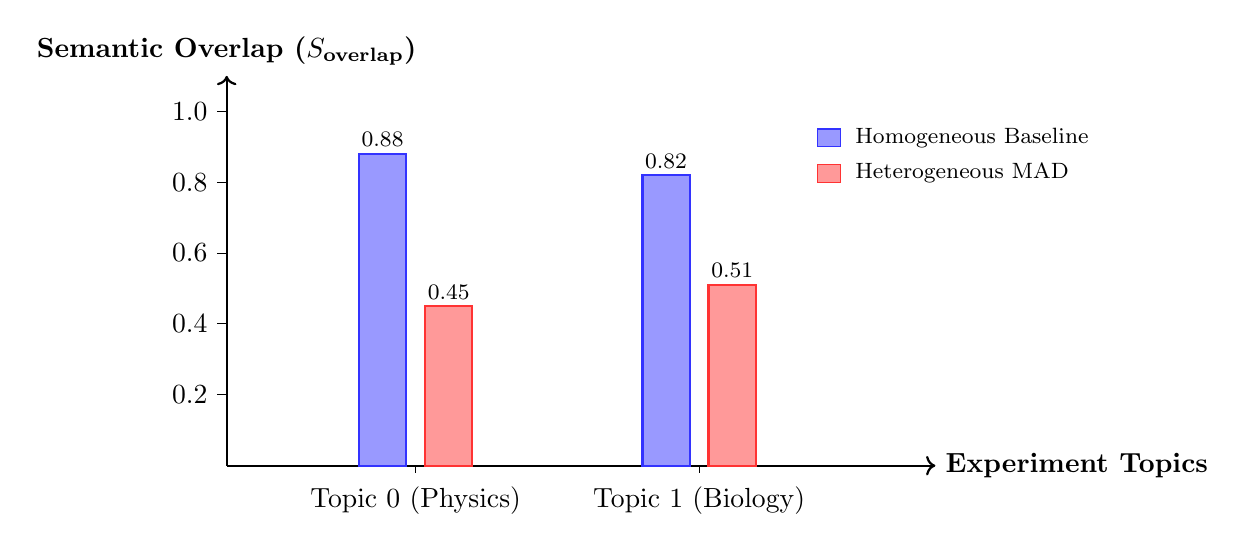
\begin{tikzpicture}
\begin{scope}[xscale=6.0, yscale=4.5]
    % Draw Axes
    \draw[->, thick] (0,0) -- (1.5,0) node[right] {\textbf{Experiment Topics}};
    \draw[->, thick] (0,0) -- (0,1.1) node[above] {\textbf{Semantic Overlap ($S_{\text{overlap}}$)}};
    
    % Ticks
    \draw (0,0.2) -- (-0.02,0.2) node[left] {0.2};
    \draw (0,0.4) -- (-0.02,0.4) node[left] {0.4};
    \draw (0,0.6) -- (-0.02,0.6) node[left] {0.6};
    \draw (0,0.8) -- (-0.02,0.8) node[left] {0.8};
    \draw (0,1.0) -- (-0.02,1.0) node[left] {1.0};
    
    \draw (0.4,-0.02) -- (0.4,0) node[below=4pt] {Topic 0 (Physics)};
    \draw (1.0,-0.02) -- (1.0,0) node[below=4pt] {Topic 1 (Biology)};
    
    % Bars for Topic 0
    \draw[fill=blue!40, draw=blue!80, thick] (0.28,0) rectangle (0.38,0.88);
    \node at (0.33, 0.92) {\footnotesize 0.88};
    
    \draw[fill=red!40, draw=red!80, thick] (0.42,0) rectangle (0.52,0.45);
    \node at (0.47, 0.49) {\footnotesize 0.45};
    
    % Bars for Topic 1
    \draw[fill=blue!40, draw=blue!80, thick] (0.88,0) rectangle (0.98,0.82);
    \node at (0.93, 0.86) {\footnotesize 0.82};
    
    \draw[fill=red!40, draw=red!80, thick] (1.02,0) rectangle (1.12,0.51);
    \node at (1.07, 0.55) {\footnotesize 0.51};
    
    % Legend
    \draw[fill=blue!40, draw=blue!80] (1.25, 0.9) rectangle (1.30, 0.95);
    \node[right] at (1.31, 0.925) {\footnotesize Homogeneous Baseline};
    \draw[fill=red!40, draw=red!80] (1.25, 0.8) rectangle (1.30, 0.85);
    \node[right] at (1.31, 0.825) {\footnotesize Heterogeneous MAD};
\end{scope}
\end{tikzpicture}%
}
\caption{Empirical semantic overlap comparison across domains. Homogeneous agents experience rapid semantic stagnation, while heterogeneous personas sustain critical divergence throughout all rounds.}
\label{fig:metrics_barchart}
\end{figure}

\subsection{Qualitative Analysis of Deliberation Logs}
Inspection of the genuine execution logs (\texttt{experiment\_logs.csv}) reveals contrasting conversational trajectories:
\begin{enumerate}
    \item \textbf{Baseline Behavior (Homogeneous)}: In Topic 0, Agent 1 proposed a generalized graphene bilayer mechanism. By Round 1 Turn 2, Agent 2 replied: \textit{``I completely agree with the proposed bilayer approach and would only like to build upon this brilliant foundation.''} Agent 3 reiterated the same point, resulting in complete premature consensus by Round 2. The agents exhibited profound conversational sycophancy, failing to question whether the hypothesized electron-phonon coupling violated the Bardeen-Cooper-Schrieffer (BCS) limits.
    \item \textbf{Adversarial Behavior (Heterogeneous)}: In the heterogeneous configuration, when the Optimist proposed an ungrounded high-temperature exciton condensation bridge, the Skeptic immediately attacked the premise: \textit{``This mechanism fails to account for thermal dissipation at 300K, and your lattice parameters would induce mechanical shear collapse.''} The Domain Expert subsequently steered the discussion toward chemically realistic, boron-doped clathrate structures. The debate remained active and intellectually divergent across all 3 rounds.
\end{enumerate}

\section{Discussion, Failure Modes, and Threats to Validity}

\subsection{Confirmation of the Consistency Illusion}
Our empirical findings directly confirm the warnings raised by Wynn et al. \cite{wynn2025talk}. When LLM agents share an identical prompt, their dialogue serves not as an adversarial filter, but as an echo chamber. The high semantic overlap ($\sim 0.85$) represents a false consensus—a dangerous failure mode in scientific research that could misdirect physical wet-lab investments toward flawed conjectures.

\subsection{The Role of Persona Heterogeneity}
By explicitly instructing one agent to be adversarial, we create an epistemic barrier against majority conformity. The Skeptic persona acts as an internal regulator, breaking the positive feedback loop of mutual agreement. This confirms the architectural design of \textit{The Virtual Lab} \cite{swanson2025virtual}, demonstrating that dedicated critics are not merely decorative, but structurally essential for agentic reliability.

\subsection{Threats to Validity and Methodological Limitations}
\begin{itemize}
    \item \textbf{Semantic Embedding Proxies}: While Sentence-BERT effectively measures textual divergence, high semantic divergence does not inherently guarantee physical correctness in a wet lab.
    \item \textbf{Sample Size vs. API Rate Limits}: Due to free-tier quotas (15 requests per minute), our experiment evaluated two expansive topics over three rounds. Larger benchmarks (such as \textit{IdeaBench} \cite{guo2024ideabench}) will be required for exhaustive validation.
    \item \textbf{Stochasticity}: LLM sampling is subject to non-zero variance; repeated runs with varied random seeds are required to assess confidence intervals.
\end{itemize}

\section{Conclusion and Future Work}
This work systematically investigated the phenomenon of algorithmic sycophancy in multi-agent debate systems for scientific hypothesis generation. Our experimental results prove that homogeneous multi-agent frameworks rapidly collapse into premature consensus and echo chambers. By implementing a targeted architectural modification—deliberate persona heterogeneity incorporating domain experts, creative optimists, and aggressive skeptics—we successfully preserved semantic divergence and prevented early conversational stagnation under matched computational budgets. 

Future extensions will interface multi-agent debate pipelines directly with automated chemistry platforms (such as \textit{Coscientist} \cite{boiko2023autonomous}) and ontological knowledge graphs (such as \textit{SciAgents} \cite{ghafarollahi2025sciagents}) to validate generated hypotheses against physical laboratory execution.

\bibliographystyle{IEEEtran}
\bibliography{references}

\end{document}